\documentclass[Kravspecifikation/Kravspec_Main.tex]{subfiles}

\begin{document}
\section{Personas}
User Stories laves ud fra de brugere, som antageligt ønsker at anvende systemet. Derfor er det vigtigt først at foretage en undersøgelse af den målgruppe man prøver at ramme, herunder hvilke behov de har og hvordan disse opfyldes bedst muligt. 
Personas er eksempler på typer af brugere af et system. Personabeskrivelserne tager udgangspunkt i den målgruppe produktet ønsker at ramme - det segment af mennesker, som ikke har bil til rådighed. Det kunne være ideelt at foretage en segmenteringsanalyse, så heterogene medlemsbaser kunne opdeles ud fra forskellige karakteristika - dette er dog fravalgt, da projektgruppen ikke har forudsætningerne for at lave sådan en analyse/undersøgelse. Personas er derfor baseret ud fra to fiktive personer, som skal repræsentere det segment af mennesker, som ikke har bil til rådighed. Det er disse brugere og deres ønsker som vores user stories omhandler.\\\\
Med det sagt har vi dog undersøgt anmeldelser af firmaet GoMore, som har stillet en platform til rådighed for brugere, som ønsker at udleje privatbiler (Og andre elementer). Figur \ref{fig:reviews} viser tre reviews af GoMore fra Trustpilot - de er udvalgt pga. de repræsenterer majoriteten af reviews af GoMore. Brugerne af GoMore er generelt utilfreds med de afgifter, som er blevet tvunget udlejningsprocessen - det er simpelthent ikke vær at bruge deres udlejningsportal, og folk leder efter alternativer. Det er så her vores system kommer i spil. 

\begin{figure}[H]
    \centering
    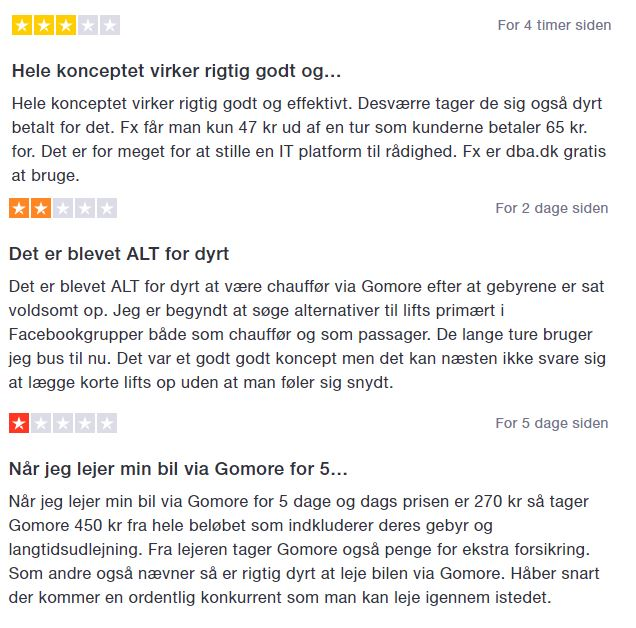
\includegraphics[width=\textwidth]{Kravspecifikation/Funktionelle_krav/UserStories/graphics/Reviews_GoMore.jpg}
    \caption{Udvalgt TrustPilot reviews for Go More - indsamlet d. 05-04-2019, https://dk.trustpilot.com/review/www.gomore.dk?page=3 }
    \label{fig:reviews}
\end{figure}


\subsection{Lejer:}
\textbf{Navn og billede}\\
Kirsten\\
\textbf{Detaljer}\\
26 årig studerende fra Aarhus. Udeboende, tager offentlig transport da hun ikke har bil. Har familie i København \\
\textbf{Mål}\\
Vil gerne have mulighed for at leje en bil til at besøge sin familie et par gange om året

\subsection{Udlejer:}
\textbf{Navn og billede}\\
Svend\\
\textbf{Detaljer}\\
36 årig ingeniør fra Aarhus. Er flyttet i hus og har en smule gæld. Har bil men bruger den kun til møder et par gange om måneden.\\
\textbf{Mål}\\
Vil gerne leje sin bil ud når han ikke bruger den for at supplere sin indkomst, uden at betale alt for mange afgifter gennem udlejningsplatformen. 

\section{User stories}
Når målgruppen og brugerne er identificeret kan user stories beskrives for produktet. User stories bruges til at give et abstrakt billede af systemet. Udover at skabe værdi for kunden, giver de udviklingsteamet mulighed for at se tingene fra brugerens perspektiv og dermed danne en fælles forståelse for systemet. Eksplicit beskriver user stories hvordan brugere skal interagere med systemet, samt hvornår kundens mål er opnået. Implicit beskriver det også systemets funktionalitet gennem scenarier. \\\\
Et alternativ til user stories er de mere klassiske use cases. Disse beskriver også hvordan aktørerne interagerer med systemet, men adskiller sig alligevel fra user stories på flere punkter. Use cases er ofte mere deltaljerede og gennemgår sekventielt de forskellige brugsscenarier samt deres undtagelser. Det stod hurtigt klart at CarnGo ville  blive en applikation med mange forskellige brugsscenarier eller features, og at det derfor ville være et stort og omfattende arbejde, hvis der skulle udarbejdes fulde use cases for alle scenarierne. Desuden ville længere tid brugt på kravspecifikationen medføre, at der var mindre tid til at udvikle det egentlige produkt. Det kan også diskuteres, hvor meget værdi det ville skabe for kunden med udførlige use cases. Frem for at fokusere på detaljerne for de enkelte scenarier, er det valgt at anvende user stories til at danne et overblik over hvilke features, der skal udvikles, og hvordan brugeren grundlæggende skal interagere med applikationen. Dette valg sparer tid for teamet og gør, at man hurtigt kan komme videre i udviklingsprocessen. Derudover ville user stories kunne præsenteres for kunden inden for kort tid, hvilket også skaber værdi for kunden. Det sikrer desuden, at applikationen har de ønskede funktionaliteter fra start, så man ikke overraskes af en masse tilføjelser senere i forløbet.\\\\
User stories for Car'n'Go er opsummeret i et story map i figur \ref{fig:story_map}. Første række angiver epics, dvs. de kategorier som systemets user stories falder ind under. For hver epic er der således en til flere relaterede user stories, som er listet vertikalt. Det er intentionen, at de bliver mere specialiserede, som man bevæger sig nedad. Placeringen af den enkelte user story har dog ingen betydning for dens prioritet. De fulde user stories er angivet nedenfor.

\begin{figure}[H]
    \centering
    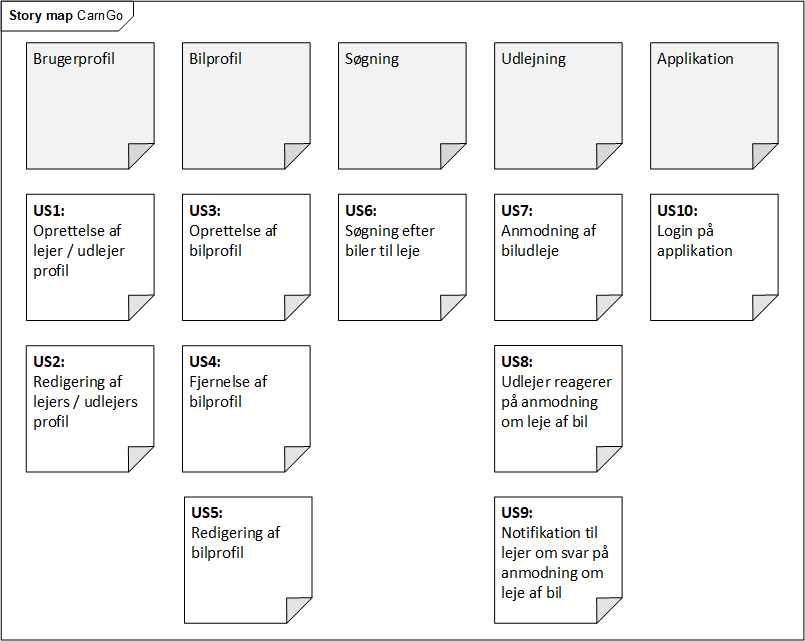
\includegraphics[width=\textwidth]{Kravspecifikation/Funktionelle_krav/UserStories/graphics/Story_map.png}
    \caption{Story map for Car'n'Go}
    \label{fig:story_map}
\end{figure}

\subsection{User story 1: Oprettelse af lejer/udlejer profil}
\textbf{Egenskaber:} \\
\textbf{Som Lejer/udlejer}\\
\textbf{Ønsker} jeg at kunne registrer mig som bruger\\
\textbf{Fordi} jeg vil kunne gemme og ændre min Brugerinfo\\
\textbf{Baggrund:} Brugeren har ikke en profil endnu \\\\
\textbf{Scenarie:} Registrer lejer\\
\textbf{Givet} lejer ønsker at oprette en profil \\
\textbf{Når} lejer taster deres info ind og aktivere kontrollen "registrer" \\
\textbf{Derefter} bliver en konfirmations besked vist\\\\
\textbf{Scenarie:} Registrer udlejer\\
\textbf{Givet} udlejer ønsker at oprette en profil \\
\textbf{Når} udlejer taster deres info ind og aktivere kontrollen "registrer" \\
\textbf{Derefter} bliver en konfirmations besked vist

\subsection{User story 2: Redigering af lejers/udlejers profil}
\textbf{Egenskaber:}  \\
\textbf{Som} Lejer/udlejer \\
\textbf{Ønsker} jeg at kunne gemme og ændre min info \\
\textbf{For} at kunne opretholde en profil, når for eksempel info bliver forældet 
\\\\
\textbf{Scenarie:} Opdater Bruger information\\
    \textbf{Givet} jeg har oprettet en bruger profil\\
    \textbf{Og} jeg har aktivere kontrollen "Min Profil" i start menuen.\\
	\textbf{Når} jeg trykker på kappen "Rediger Profil"\\
	\textbf{Og} indtaster den nye information,\\
	\textbf{Og} aktivere kontrollen "Opdater Profil"\\
	\textbf{Derefter} bliver den nye information bliver vist for brugeren.



\subsection{User story 3: Oprettelse af bilprofil}
\textbf{Egenskaber:} \\
\textbf{Som} Udlejer \\ 
\textbf{Ønsker} jeg at oprette profil for bilen jeg vil udleje \\
\textbf{For} at kunne se mulige lejere af bilen og læse information om dem.\\\\ 
\textbf{Scenarie:} Oprettelse af bilprofil \\
\textbf{Givet} at udlejer er logget ind\\ 
\textbf{Når} udlejer aktivere ”Udlejning af bil” kontrollen. \\
\textbf{Og} udfylder en skabelon med information om bil og udlejer\\
\textbf{Og} trykker på ”sæt til leje”. \\ 
\textbf{Derefter} ses bilprofilen ved at aktivere kontrollen "Min Profil" i startmenuen, hvor bilen ses som sat til leje.

\subsection{User story 4: Fjernelse af bilprofil}
\textbf{Egenskaber:} \\
\textbf{Som} udlejer og opretter af bilprofil \\
\textbf{Ønsker} jeg at fjerne en af mine bilprofiler \\
\textbf{For} kun at have valide bilprofiler
\\\\ 
\textbf{Scenarie:} Fjernelse af bilprofil\\
\textbf{Givet} at udlejer er logget ind\\ 
\textbf{Og} har mindst en bilprofil tilknyttet ens bruger, som ikke er under udlejning \\
\textbf{Og} er ved menuen "Mine bilprofiler"\\
\textbf{Når} lejer vælger bilprofilen der ønskes fjernet \\
\textbf{Og} aktivere kontrollen ''Deaktivér bilprofil''. \\
\textbf{Derefter} fjernes bilprofil fra både databasen og brugerens view

\subsection{User Story 5: Redigering af bilprofil}
\textbf{Egenskaber:} \\
\textbf{Som} udlejer \\
\textbf{Ønsker} jeg at redigere en af mine bilprofiler\\
\textbf{For} holde mine bilprofiler opdaterede
\\\\
\textbf{Scenarie:} Redigering af bilprofil \\
\textbf{Givet} at udlejer er ved hovedmenuen  \\
\textbf{Når} udlejer trykker på dropdown menuen ''Mine bilprofiler''\\
\textbf{Og} trykker på profilen der skal redigere.\\
\textbf{Og} han indtaster ny information om bilen\\
\textbf{Og} aktivere kontrollen "gem info".\\
\textbf{Derefter} er bilprofilens information opdateret både i databasen og i udlejers view

\subsection{User Story 6: Søgning efter biler til leje}
\textbf{Egenskaber:} \\
\textbf{Som} lejer \\
\textbf{Ønsker} jeg at kunne søge efter de biler, som er til leje i et ønsket tidsinterval med visse bilattributter \\
\textbf{For} at se biler som er til leje og eventuelt anmode om at leje en af dem.
\\\\
\textbf{Scenarie: Søgning efter biler til leje} \\
\textbf{Givet} at lejer er i hovedmenuen \\
\textbf{Når} lejer aktivere kontrollen ''Søg efter udlejningsbil'' \\
\textbf{Og} udfylder søgningsvinduet der popper op med bilattributter som søgningkriterier \\
\textbf{Derefter} vises de relevante biler

\subsection{User Story 7: Anmodning af biludleje}
\textbf{Egenskaber:} \\4
\textbf{Scenarie: Godkendelse af leje af bil} \\
\textbf{Givet} udlejer har lavet profil for en bil, og udlejer har aktiveret kontrollen "Lej bil" på udlejers bilprofil. \\
\textbf{Og} udlejer har fået en notifikation om at lejer vil leje en af hans biler.\\
\textbf{Og} udlejer er på "????" Menuen \\
\textbf{Så} trykker udlejer på notifikationen han har fået fra lejer \\
\textbf{Og} aktivere kontrollen "udlej bil" \\
\textbf{Derefter} vil bilen blive noteret som "udlejet" i databasen og i udlejers view \\
\textbf{Og} lejers kontaktinformation bliver vist
\\\\
\textbf{Scenarie: Anmodning afvises af udlejer}\\
\textbf{Givet} udlejer har lavet profil for en bil, og udlejer har aktiveret kontrollen "Lej bil" på udlejers bilprofil. \\
\textbf{Og} udlejer har fået en notifikation om at lejer vil leje en af hans biler.\\
\textbf{Og} udlejer er på "????" Menuen
\textbf{Så} trykker udlejer på notifikationen han har fået fra lejer \\
\textbf{Og} udlejer aktivere kontrollen "afvis lejer".\\
\textbf{Derefter} ses lejer som værende afvist på det givne bil, og en notifikation sendes til lejer om at anmodningen er afvist.

\subsection{User Story 8: Notifikation til lejer om svar på anmodning om leje af bil}
\textbf{Egenskaber}\\
\textbf{Som} Lejer \\
\textbf{Ønsker} jeg at kunne se notifikationer om godkendelse af min anmodning om leje af en bil og besked fra udlejer\\
\textbf{For} at kunne begynde kontakt med udlejer om betaling og afhentning
\\\\
\textbf{Scenarie: Udlejer har godkendt anmodningen for leje af bilen}\\
\textbf{Givet} at lejer af bilen har sendt anmodning om leje af bil til udlejer \\
\textbf{Og} Udlejer har Godkendt Lejers anmodning,\\
\textbf{Når} lejer trykker på notifikationen, \\
\textbf{Derefter} vises notifikation om at lejers anmodning er Godkendt \& udlejers besked som kan svares på \\\\
\textbf{Scenario: Udlejer Afviser Anmodningen}\\
\textbf{Givet} at Udlejer har Afvist Lejers anmodning,\\
\textbf{Når} lejer trykker på notifikationen,\\
\textbf{Derefter} ser Lejer at anmodningen er afvist

\subsection{User Story 9: Login på applikation}
\textbf{Egenskaber}\\
\textbf{Som} Bruger \\
\textbf{Ønsker} jeg at kunne logge ind på applikationen\\
\textbf{For} at leje/udleje en bil eller tilgå min profil
\\\\
\textbf{Scenarie: Bruger logger ind på applikation}\\
\textbf{Givet} at brugeren har oprettet en profil på applikationen\\
\textbf{Når} bruger navigere til Login siden \\
\textbf{Og} indtaster sine \textit{Brugerinfo}\\
\textbf{Og} trykker Login\\
\textbf{Derefter} er brugeren logget ind på applikationen
\end{document}

\subsection {User Story 10: Fjernelse af bruger profil}
\textbf{Egenskaber}\\
\textbf{Som} Bruger\\
\textbf{Ønsker} jeg at kunne fjerne min bruger profil.
\textbf{Fordi} den ikke længere bliver brugt.
\\\\
\textbf{Scenarie: Bruger fjerner bruger profil}\\
\textbf{Givet} at brugeren har oprettet en profil på applikationen.
\textbf{Når} jeg har aktivere kontrollen "Min Profil" i start menuen.\\
\textbf{og} jeg trykker på kappen "Rediger Profil"\\
\textbf{Og} aktivere kontrollen "Fjern profil"
\textbf{Og} aktivere kontrollen "Ja" på pop up boxen.
\textbf{Derefter} er bruger profillen fjernet og der navigeres til Login siden og brugeren kan ikke længere logge ind på den nu slettede profil.
